
\documentclass[10pt]{article}
% Эта строка — комментарий, она не будет показана в выходном файле
\usepackage{ucs}
\usepackage[utf8x]{inputenc} % Включаем поддержку UTF8
\usepackage[russian]{babel}  % Включаем пакет для поддержки русского языка
\usepackage{amsmath}
\usepackage{amssymb}
\usepackage{mathtools}

\hoffset=0mm
\voffset=0mm
\textwidth=170mm        % ширина текста
\oddsidemargin=-0mm   % левое поле 25.4 - 5.4 = 20 мм
\textheight=240mm       % высота текста 297 (A4) - 40
\topmargin=-15.4mm      % верхнее поле (10мм)
\headheight=5mm      % место для колонтитула
\headsep=5mm          % отступ после колонтитула
\footskip=8mm         % отступ до нижнего колонтитула

% \textwidth=180mm    
% \oddsidemargin=-10mm 

\title{Задача об оптимальном расписании (Scheduling Problem)}
\author{Зотов Алексей, 497}
\date{\today}

\begin{document}
\maketitle
\paragraph{\Large {Формулировка задачи\\\\}} 

\indent Имеется множество работ $J$ и множество машин $M$. Также задана функция $p: J \times M \to \mathbb{R}_+$. Значение $p(i,j) = p_{ij}$ означает время выполнения $i$-ой работы на $j$-ой машине. \\
Требуется найти распределние работ по машинам, так чтобы время выполнения всех работ было минимально. Формально, требуется построить функцию $x : J \times M \to \{1,0\}$ такую, что: 
\begin{equation}
    \sum_{j \in M} x_{ij} = 1 , \quad \forall i
\end{equation}
\begin{equation}
    \max_{j \in M} \sum_{i} x_{ij} p_{ij} \to \min 
\end{equation}
\\
\\
\paragraph{\Large{$\mathbf{NP}$ - полнота\\\\}}
\indent \textbf{Теорема.} Задача об оптимальном расписании является $\mathbf{NP}$ - полной. \\
Здесь рассматривается измененный вариант задачи:
\begin{equation}
     \max_{j \in M} \sum_{i} x_{ij} p_{ij} \leq k
\end{equation} \\
{\itshape Доказательство.}
\begin{enumerate}
    \item \textbf{SCHEDULING} $\in$ \textbf{NP} \\
    \indent Действительно, сертификатом будет являться значения функции $x$ на множестве $J$. Полиномиально вычисляется искомый функционал.
    \item Рассмотрим  задачу \textbf{SUBSETSUM}. \\
    Дано множество $A$, определена весовая функция $s : A \to \mathbb{N}$ на элементах множества. Необходимо найти подмножество
    $A'\subseteq A$, такое что $\sum_{a \in A'} s(a) = \sum_{a \in A\backslash A'} s(a)$. \\
    Легко свести данную задачу к задаче о расписании, взяв $J = A$ - множество элементов как множество работ, $M = \{1,2\}$ - два подмножества в задаче о разбиении как две машины, $p_{ij} = s(a_i)$ - вес элемента как сложность выполнения работы и $k = 0$, так как нам нужно точное разбиение. Тогда, решив задачу о расписании, мы получим решение задачи о разбиении. \\
    Покажем теперь, что \textbf{SUBSETSUM} \textbf{NP} - трудна, что завершит доказательство теоремы. \\ \\ 
    \textbf{Утверждение.} \textbf{SUBSETSUM} $\in$ \textbf{NPH}. \\
    {\itshape Доказательство утверждения.} Сведем \textbf{NP} полную задачу о покрытии ребрами 3-дольного 3-однородного гиперграфаграфа 
    (\textbf{3-dimensional matching , 3DM}) к задаче \textbf{SUBSETSUM}. \\ Пусть $W = \{w_1,\dots w_q\},X=\{x_1,\dots x_q\},Y=\{y_1,\dots y_q\}$ , $V = W \cup X \cup Y$- вершины и $M \subseteq W \times X \times Y$, $|M| = k$ - ребра гиперграфа из задачи \textbf{3DM}.\\
    Будем считать, что $\forall v \in V \exists e \in M: v \in e$, то есть для каждой вершины существует ребро, которое ее содержит. Если это не так, то ответ на задачу отрицательный, и это можно вычислить за полиномиальное время. \\
    Требуется построить множество $A$ и размеры $s(a)$ всех его элементов так, чтобы было выполнено: 
    \begin{equation}
        \exists A' \in A \sum_{a \in A'} s(a) = \sum_{a \in A' \backslash A} s(a) \
        \iff \exists J \subseteq \{1\dots k\}, m_{j} \in M, j \in J : \bigsqcup_{J} m_j = V
    \end{equation}
    то есть, что в $A$ можно найти подмножество, равное по весу своему дополнению, тогда и только тогда, когда $M$ содержит искомое покрытие. \\
    Множество $A$ будет состоять из $k+2$ элементов. Первые $k$ элементов множества $A$ будут $\{ a_i: 1 \leq i \leq k\}$, вес элемента $s(a_i)$ будет определеяться по $m_i$. Построим двоичную запись числа $s(a_i)$ по $m_i = (w_{f(i)},x_{g(i)},y_{h(i)})$. Для записи $s(a_i)$ будем использовать ровно $3qp$ бит, где $p = \lceil \log_2{(k+1)} \rceil$. Каждой из трех компонент $m_i$ соответствует один подотрезок длины $qp$ в двоичной записи числа $s(a_i)$, который состоит из $q$ блоков длины $p$, каждый блок соответствует своему $1 \leq i \leq q$. В числе $s(a_i)$ правые концы зон, соответствующих $w_{f(i)}, x_{g(i)}, y_{h(i)}$ равны 1, остальные биты равны 0:
    \begin{equation}
        s(a_i) = 2^{p(3q - f(i))} + 2^{p(2q - g(i))} + 2^{p(q - h(i))}
    \end{equation}

    $s(a_i)$ имеет длину не больше $3pq$, и может быть построено за полиномиальное время.
    \begin{center}
        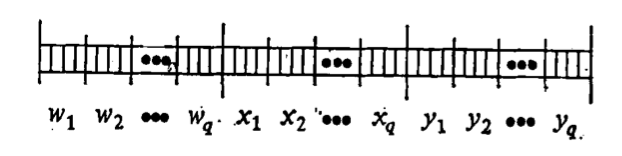
\includegraphics[height=2cm]{img1.png} \\ $s(a_i)$
    \end{center}
    Заметим, что если просуммировать содержимое одной зоны всех элементов множества $\{a_i: 1 \leq i \leq k\}$, то результат не будет превосходить $2^p - 1$. Следовательно, при суммировании по любому подмножеству, никогда не придется переносить единицы из одной зоны($p$ бит) в соседнюю. \\
    Положим :
    \begin{equation}
        B = \sum^{3q-1}_{j=0} 2^{pj}
    \end{equation}
    $B$ - число, в двоичной записи которого в правом конце каждой зоны стоит 1. Тогда для любого подмножества 
    $A' \subseteq \{a_i: 1 \leq i \leq k\}$, соотношение: 
    \begin{equation}
        \sum_{a \in A'} s(a) = B
    \end{equation}
    выполняется тогда и только тогда $M' = \{m_i :a_i \in A'\}$ - решение \textbf{3DM}.
    Последние два элемента $b_1$ и $b_2$ множества $A$ такие, что выполнено:
    \begin{equation}
        s(b_1) = 2 \left( \sum^{k}_{i=1}s(a_i) \right) - B
    \end{equation}
    \begin{equation}
        s(b_2) = \left( \sum^{k}_{i=1}s(a_i) \right) + B
    \end{equation}
    Двоичные записи $s(b_1)$ и $s(b_2)$ имеют длину не более $3pq + 1$ и могут быть построены за полиномиальное время.

    Предположим, что имеется подмножество $A' \subseteq A$, такое, что: 
    \begin{equation}
        \sum_{a \in A'} s(a) = \sum_{a \in A' \backslash A} s(a)
    \end{equation}
    Тогда каждая из этиъ сумм должна быть равна $\frac{1}{2} \sum_{a \in A} s(a) = 2 \sum^{k}_{i=1} s(a_i)$.
    Также $s(b_1) + s(b_2) = 3 \left(\sum^{k}_{i=1} s(a) \right)$, значит одно из множеств $A'$ или 
    $A' \backslash A$ содержит $b_1$ и не содержит $b_2$. Значит остальные элементы этого подмножества из $\{a_i: 1 \leq i \leq k \}$ и сумма их весов в точности равна $B$. Тогда, по сделанному ранее замечанию, этому подмножеству соответствует $M' \subseteq M$ являющееся решением задачи \textbf{3DM}. \\ 
    Обратно, если задано покрытие $M' \subseteq M$, являющееся решением задачи \textbf{3DM}, то ${b_1} \cup {a_i:m_i \in M'}$ - искомое множество $A'$. \\
    Утверждение даказано, и тем самым даказана теорема об \textbf{NP} - полноте задачи о расписании.




\end{enumerate}
\paragraph{\Large{Полиномиальное приближение\\\\}}
\indent Найдем полиномиальное приближенное решение для частного случая задачи об оптимальном рассписании, когда мощности всех машин одинаковы, то есть $p_{ij} = p_i$. \\ \\ 
Рассмотрим алгоритм \textbf{LPTR} (Longest Processing Time Rule): \\
\begin{enumerate}
    \item Отсортируем работы в порядке невозрастания сложности работы $p_i$, то есть так, что $p_i \geq p_{i+1} \quad \forall i$. 
    \item Пройдем все работы в данном порядке, назначая на $i$-м шаге данную работу той машине, которая завершит обработку уже назначенных ей задач раньше всех остальных машин.
\end{enumerate}

\indent \textbf{Теорема.} LPTR - имеет коэффициент аппроксимации $\frac{4}{3}$ для задачи об оптимальном расписании, 
то есть $ \text{LPTR} (x) \leq \frac{4}{3} \text{OPT} (x) \quad \forall x$ - входные данные , $\text{OPT} (x)$ - оптимальное решение. \\
\indent $\triangleleft$ 
                Пусть $S$ - расписание, результат работы \textbf{LPTR} алгоритма, $w(S)$ - время окончания работ. Пусть $l$ - работа, которая завершится последней. Можно считать, что $l$ - это номер последней работы. Если это не так,
                то докажем для $J' = \{1 \cdots l\}$. Тогда для новой и исходной задачи алгоритм выдаст расписание с одним и тем же временем окончания работы, то есть $w(S') = w(S)$, в то время как оптимальное время в исходной задаче может быть только больше либо равно оптимальному времени в новой задаче ($\text{OPT} \geq \text{OPT}'$). Значит, доказав аппроксимацию для работы на $J'$, автоматически докажем и для работы на $J$. \\

                Пусть $t_l$ - время начала выполнения работы $l$. Тогда в этот момент времени все машины заняты (одна или несколько могли освободиться в данный момент), иначе если какая-то машина была свободна, то  $t_l$ было бы меньше (в момент времени $t = 0$ все машины считаются занятыми). Значит все время $t_l$ все $m$ машин работали непрерывно: 
                \begin{equation}
                    t_l \leq (\sum_{j \in M} p_j - p_l)/m \leq \text{OPT} - \frac{p_l}{m}
                \end{equation}

                \begin{equation} \label{eq:estimation}
                    w(S) = t_l + p_l \leq \text{OPT} + p_l (1 - \frac{1}{m}) 
                \end{equation}

                \textbf{Лемма.} Если $p_{\min} > \frac{\text{OPT}}{3}$, то $w(S) = OPT$. \\
                \indent {\itshape{Доказательство леммы.}} В условиях леммы в оптимальном расписании будет не более двух задач на одной машине. Покажем что LPTR алгоритм также не назначит более двух задач на одну машину. Всего работ не более чем $2m$. Предположим в $S$ на какой-то машине не менее 3х работ. Пусть $k$ - первая работа которая стала 3-ей на какой-то машине. Тогда есть и работа $j$, которая единственна на своей машине в $S$  
                и не единственна в оптимальном. Заметим, что в LPTR $j$ будет рассмотрена раньше $k$ , иначе $k$ была бы распределена на свободную машину. Тогда $p_j < 2 \text{OPT} /3 $. С другой стороны, $p_j > 2 p_{\min} > 2 \text{OPT}/3$, иначе работа $k$ могла бы быть распределена на машину к работе $j$. Значит $LPTR$ назначает не более двух работ на машину. Можно найти такое оптимальное расписание $S_2$, что $a_i \geq a_j \quad i \leq j$ и $b_i \leq b_j \quad i \leq j$, где $a_i$ и $b_i$ - время обработки первой и второй работ соответственно на $i$-ой машине. Именно такое расписание и выдаст LPTR алгоритм.

                {\itshape Завершим доказательство теоремы.} \\
                Если $p_{\min} > \frac{\text{OPT}}{3}$, то $S$ - оптимальное расписание. Иначе $p_l \leq \frac{\text{OPT}}{3}$ 
                и по (\ref{eq:estimation}) получаем :
                \begin{equation}
                    w(S) \leq \text{OPT} + \frac{\text{OPT}}{3} (1 - \frac{1}{m}) \leq \frac{4}{3} \text{OPT}
                \end{equation}
                Что завершает доказательство. $\triangleright$

\paragraph{\Large{Тесты\\\\}}
Проверим работу алгоритма, рассмотрев несколько тестов. \\ 
input:\\
N = 6, M = 2, a = [2, 3 ,5, 2, 2, 2].\\
output:\\
W = 9; S = [0 1 0 1 0 1] $\neq$ OPT, OPT = 8, так как(5 + 3 = 2 + 2 + 2 + 2). \\ \\ 
input: \\
N = 10, M = 3, a = [1, 2, 3, 4, 5, 6, 7, 8, 9, 10] \\
output: \\
W = 19; S = [2 2 1 0 0 1 2 2 1 0] - оптимальный ответ, т.к. OPT > $1/n \sum a_i$ = 18.33 >= 19 \\ \\ 
input: \\
N = 4, M = 2, a = [8 2 7 3] \\
output:\\
W = 10; S = [0 0 1 1] = W(OPT). \\ \\
input: \\N = 10, M = 3, a = [1,2,3,4,5,6,7,8,9,10]\\
output: \\
W = 19 = W(OPT); S = [2 2 1 0 0 1 2 2 1 0]
\\\\
Сгенерируем большой случайный тест: \\
input: \\
N = 100, M = 3, a = $[81, 97, 64, 54, 72, 83, 0, 17, 44, 84, 59, 67, 58, 81, 94, 10, 62, 36, 52, 91, 0, 89, 97, 12, 60, 87, 54, 27, 18, 75, 79, 97, 84, 92, 89, 22, 70, 82, 12, 50, 23, 27, 73, 23, 56, 92, 61, 14, 90, 97, 23, 68, 57, 26, 87, 32, 40, 32, 13, 74, 64, 9, 35, 1, 21, 60, 55, 24, 75, 35, 47, 87, 1, 17, 5, 65, 68, 55, 8, 43, 70, 94, 42, 33, 40, 55, 86, 96, 26, 44, 13, 63, 94, 77, 98, 25, 19, 68, 15, 6]$
output: \\ 
W = 1750, S = [2 2 0 2 0 1 2 0 2 2 1 0 2 0 2 2 2 0 0 2 2 1 1 1 0 2 2 2 2 0 0 2 1 1 0 1 2 2 0 1 2 1 1 0 1 0 1 1 2 1 2 1 2 2 1 0 2 2 2 2 2 0 1 1 0 0 1 1 1 1 1 0 2 0 1 2 0 0 0 0 2 1 1 0 2 0 0 0 1 0 1 1 0 1 0 0 1 1 2 2], \\
$1/3 \sum a_i = 1749.66 \implies W(\text{OPT}) >= 1750 \implies W = W(\text{OPT}).$ \\ 
На случайных данных алгоритм работает хорошо и с большой вероятностью дает точное решение.


\paragraph{\Large{Список литературы\\\\}}
\begin{itemize}
 \item $[1]$ http://research.microsoft.com/en-us/um/people/dechakr/Courses/CO454/Lectures/lecture12.pdf
 \item $[2]$ М.Гэри, Д.Джонсон "Вычислительные машины и труднорешаемые задачи". М.: Мир, 1982.
\end{itemize}

\end{document}